\documentclass[11pt]{letter}

\usepackage{graphicx}
\usepackage{pdfpages}
\usepackage{array}
\usepackage{float}

\begin{document}

% \maketitle

Tatiana Balbi Fraga \\
Flat Club Meridional, APT. B1-2PS, AV. BEIRA MAR,  \\
PRAIA DOS CARNEIROS - TAMANDARÉ - PE CEP 55578-000 \\
tbfraga@proton.me \\

23/04/2024

Juizo de Direito da Vara Única da Comarca de Tamadaré \\
Rua Dr. Leopoldo Lins, S/N, Centro, \\
Tamandaré - PE. CEP:55578-000

Assunto: Contestação à Ação Monitória nº 0001346-98.2022.8.17.3450

Prezado(a) Senhor(a) Juiz(a),

Eu, TATIANA BALBI FRAGA,
brasileira, professora universitária, solteira, inscrita no Cadastro de Pessoas Físicas sob o número 073.815.927-11, e com cédula de identidade de nº 108.229.303 SECC-RJ, venho, por meio deste documento, apresentar minha contestação à Ação Monitória proposta por MONTEBALITO BRASIL EMPRRENDIMENTOS IMOBILIÁRIOS LTDA, atual
denominação da METAMBIENTE BRASIL EMPREENDIMENTOS IMOBILIÁRIOS LTDA, neste documento referido como AUTOR ou METAMBIENTE, nos termos do artigo 702 e seguintes do Código de Processo Civil.

1. DO ENDEREÇO DA RÉ

Peço que o ENDEREÇO DA RÉ que consta nos autos seja substituído por: FLAT CLUB MERIDIONAL, APT. B1-2PS, AV. BEIRA MAR, PRAIA DOS CARNEIROS - TAMANDARÉ - PE CEP 55578-000. 

Motivo: conforme é sabido pelo AUTOR, sou proprietária do apartamento B1-2PS do CONDOMÍNIO FLAT CLUB MERIDIONAL, que é o imóvel cujo financiamento é discutido neste processo. Conforme é conhecido por lei, os funcionários do condomínio podem receber citação em meu nome, sendo portanto obrigados a me informar imediatamente sobre qualquer citação. Não compreendo porque o AUTOR não informou o endereço do imóvel objeto de cobranças nos autos deste processo. 

2. DOS FATOS:

2.1 SOBRE O FINANCIAMENTO

Alega o AUTOR que sou devedora da quantia de 113.178,72 reais referente ao contrato CONTRATO DE COMPRA E VENDA DO APARTAMENTO B1-2PS DO CONDOMÍNIO FLAT CLUB MERIDIONAL, datado de 03/02/2011, celebrado entre as partes. Contudo, eu contesto veementemente a existência de qualquer dívida com o AUTOR, devido aos fatos apresentados a seguir.

De acordo com QUADRO RESUMO da PROMESSA DE COMPRA E VENDA celebrada entre as partes e já acostada aos autos, o apartamento B1-2PS do CONDOMÍNIO FLAT CLUB MERIDIONAL, que eu comprei, estava previsto para ser entregue em 29/12/2014. Conforme cópias de e-mails anexadas neste processo, no final do ano de 2014 eu entrei em contato com o banco CAIXA ECONÔMICA através de correspondente bancária indicada pela própria METAMBIENTE e realizei solicitação de avaliação de crédito para já obter o financiamento em dezembro do mesmo ano, momento em que o apartamento deveria estar pronto para entrega. Contudo, a correspondente bancária do banco CAIXA ECONÔMICA me informou que para liberar o financiamento, seria necessário um documento do imóvel denominado Habite-se, o qual pode ser obtido unicamente pela empresa junto à prefeitura após o momento em que o imóvel encontra-se pronto para ser habitado.

Eu enviei e-mail para a empresa METAMBIENTE informando que eu estava aguardando o Habite-se para obter o financiamento e solicitei que me informassem quando a empresa estivesse em posse do Habite-se. Ressalto que até então todos os contatos que tive com a empresa, incluindo o recebimento das faturas para pagamento das prestações, eram realizados através de e-mail.

Conforme mostra documento em anexo, eu fui informada sobre a finalização do imóvel apenas em 29/06/2015, quando eu estive na empresa para questionar sobre a disponibilidade do Habite-se, necessário para o financiamento da parcela final e recebimento do imóvel. A empresa me informou que o imóvel já estava pronto desde abril do mesmo ano, mas no entanto, até aquele momento eles não me informaram sobre o Habite-se. Apenas me enviaram um e-mail informando sobre unidade quase pronta. Conforme documentos anexados a este processo, é possível verificar que o valor cobrado em 29/06/2015 para quitação do pagamento do imóvel através de financiamento do imóvel foi de 188.501,17 reais.

Neste momento procurei novamente o banco CAIXA ECONÔMICA para realizar o financimanto, mas este não estava mais aprovando financiamentos de imóveis do CONDOMÍNIO FLAT CLUB MERIDIONAL, tendo em vista que o condomínio possui uma área de reserva da marinha. Então, em seguida procurei o Banco Real sob recomendação da pŕopria METAMBIENTE, mas não consegui fazer o financimaneto através deste banco devido às exigencias do mesmo. Então procurei o BANCO BRADESCO. O BANCO BRADESCO me entregou documento com a relação de todos os documentos exigidos para financiamento do imóvel, incluindo documentos meus assim como documentos do imóvel e documentos da empresa, que seriam de responsabilidade do AUTOR. Entreguei ao banco todos os meus documentos solicitados, e solicitei ao AUTOR, na época METAMBIENTE BRASIL EMPREENDIMENTOS IMOBILIÁRIOS LTDA, os documentos do imóvel e os documentos da empresa, conforme recomendação do próprio banco. Como sou funcionária federal e na época não tinha nenhum outro empréstimo ou qualquer limitação de crédito, rapidamente eu tive a aprovação do crédito, contudo para conseguir o financiamento, era necessário entregar ao banco os documentos da empresa e do imóvel.

Conforme mostra imagem abaixo o Habite-se só foi averbado pela empresa METAMBIENTE em 28/10/2015.

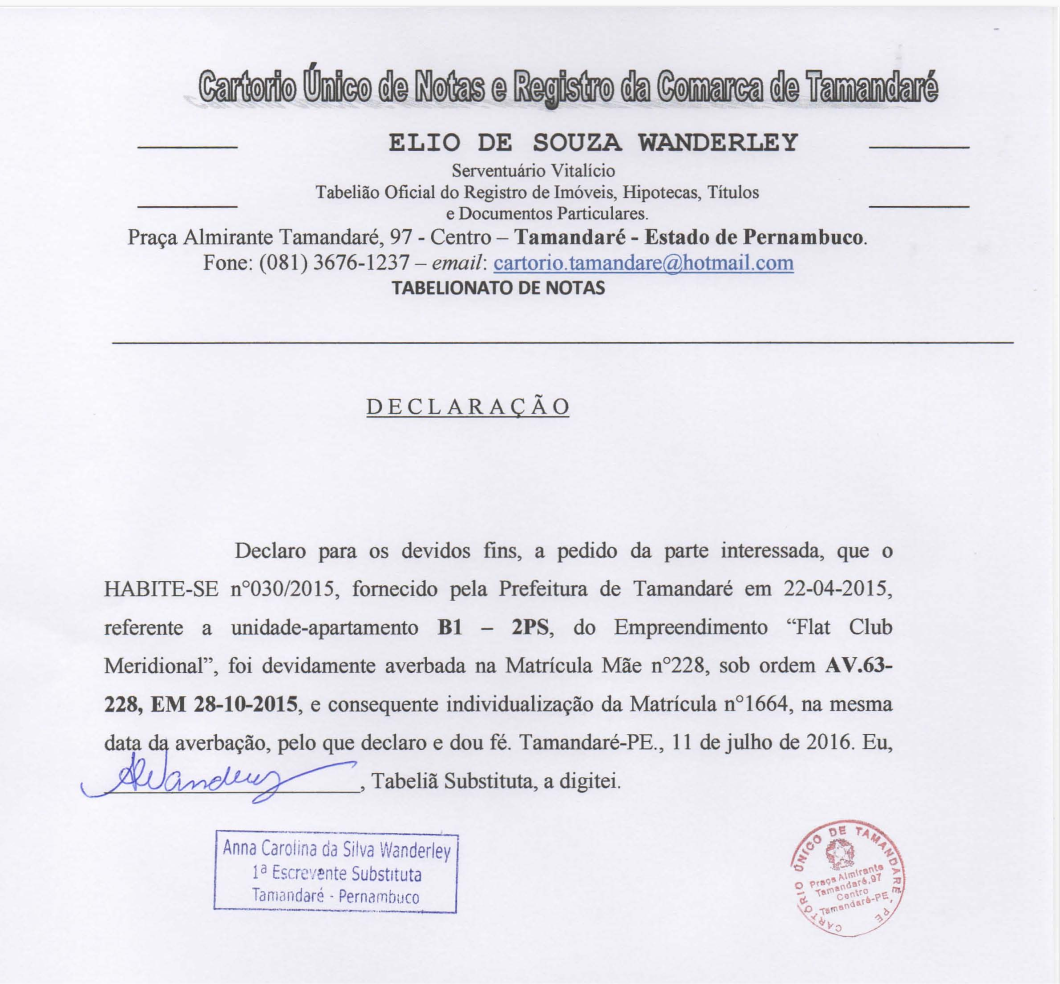
\includegraphics[width=\textwidth]{doc.png}

A averbação do Habite-se era responsabilidade da METAMBIENTE. Até onde eu saiba a averbação do Habite-se é um procedimento necessário para o financiamento do imóvel em qualquer banco. Portanto não seria possível realizar o financimanto antes desta data (28/10/2015).

Quando a METAMBIENTE me entregou o último documento solicitado pelo BANCO BRADESCO, o qual dependia da averbação do Habite-se, eu repassei este documento imediatamente para o BANCO BRADESCO. O BANCO BRADESCO então marcou uma visita técnica diretamente com a própria METAMBIENTE para avaliação do imóvel. Depois eu soube que a avaliação do imóvel foi reprovada pelo engenheiro contratado pelo BANCO BRADESCO para tal finalidade, porque o imóvel não estava identificado. O banco solicitou uma planta do condomínio com a identificação dos imóveis à METAMBIENTE para poder resolver este problema, mas a empresa não entregou o documento solicitado ao banco. 

Quando eu soube do ocorrido, fiz todo o possível para resolver o problema. Conversei com o gerente responsável e pedi à empresa METAMBIENTE que colocasse uma placa com a devida identificação do imóvel próximo à porta do apartamento a ser financiado, conforme solicitação do gerente responsável. 

Contudo, a empresa METAMBIENTE não atendeu à minha solicitação. Eu acabei perdendo a paciência e fiz uma placa para colocar pessoalmente. Contudo ao falar com a empresa sobre minha atitude planejada, a METAMBIENTE providenciou a identificação do imóvel. 

Logo em seguida solicitei nova visita técnica, depois disso o banco solicitou novamente os documentos. Novamente a empresa METAMBIENTE criou dificuldades. Inclusive solicitou que eu pagasse funcionário para adiquirir novamente os documentos. Após me entregarem documentação necessária, o financiamento seguiu os trâmites normais e foi finalmente aprovado. O que atrasou o financiamento foram a demora na entrega da documentação do imóvel e da empresa, responsabilidades da METAMBIENTE, assim como a reprovação da primeira visita técnica. 

É necessário verificar que na CLAUSULA III - DA COMPRA E VENDA do Instrumento Particular de Financiamento assinado pela empresa Metambiente Brasil Empreendimentoa Imobiliarios, por mim, Tatiana Balbi Fraga, e pelo Banco Bradesco,  consta no ponto 3.2 que o VENDEDOR DA AO COMPRADOR PLENA, GERAL E IRREVOGÁVEL QUITAÇÃO E TRANSFERE AO COMPRADOR DESDE JÁ A POSSE E DOMINIO DO IMÓVEL ... 

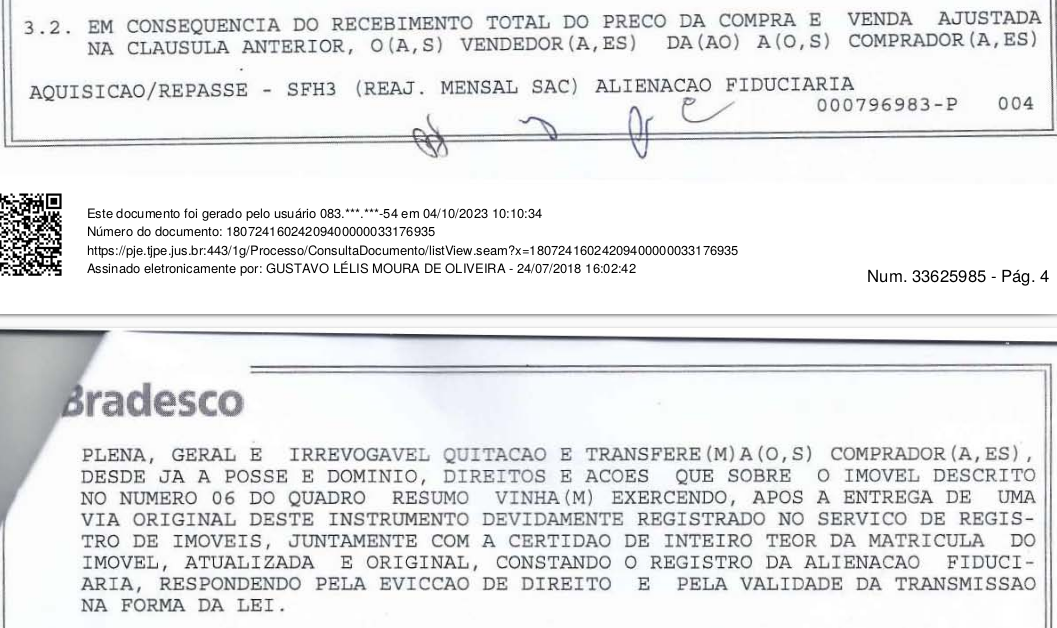
\includegraphics[width=\textwidth]{doc2.png}

Contudo, após o financiamento, a empresa se negou à me entregar as chaves do imóvel, me coagindo à pagar um valor que a empresa alega que eu devia. Devido à cobrança, eu solicitei à empresa METAMBIENTE fatura para pagamento mas a empresa não me entregou qualquer fatura. Ao invés disso, a empresa METAMBIENTE condicionou a entrega das chaves do imóvel à assinatura de um termo de confissão de dívida. Eu solicitei a fatura com o intuito de procurar um advogado para saber se de fato eu devia algum valor à METAMBIENTE. Caso algum advogado me informasse que o valor era de fato devido eu iria negociar o pagamento com a METAMBIENTE, contudo, assinando um termo de dívida, eu estaria assumindo uma dívida que eu acredito não existir. 

Ademais a empresa alegou que, mesmo sem eu receber as chaves do imóvel, eu era responsável pelo pagamento do condomínio e de outras cobranças, tal como o IPTU. Durante um longo período eu paguei todas as taxas e cobranças do imóvel, sem no entanto ter recebido às chaves deste.

Entendendo que caso houvesse uma dívida, na época logo após o financimento, a empresa METAMBIENTE poderia simplesmente me enviar fatura com a cobrança e, caso eu não pagasse, esta poderia ainda entrar com um processo de cobrança na justiça. Mas a METAMBIENTE optou por me coagir, me forçando e entrar com um processo na justiça para solicitação das chaves do imóvel.

De acordo com contrato, eu deveria ter recebido o meu imóvel em 29/12/2014, contudo só fui ter acesso ao meu imóvel em 15/01/2019, através de liminar da justiça e de mandato de imissão de posse. 

2. DA PRESCRIÇÃO DE DÍVIDAS

O contrato de financiamento e quitação do imóvel foi firmado em 27/04/2016. Portanto, com base no artigo 206 da Lei nº 10.406 de 10 de Janeiro de 2002, caso este juizo entenda que existe alguma dívida pendente a ser paga por mim, solicito que esta seja considerada prescrita.

3. DA MÁ FE DA PARTE AUTORA

Apesar de ter pleno conhecimento sobre os fatos, o AUTOR tem má fé ao omitir sua responsabilidade por ter provocado atrasos no financiamento, principalmente em função de sua negligência na entrega de documentação necessária para o financiamento solicitada pelo BANCO BRADESCO.

A empresa também tem má fé ao reter as chaves do imóvel para tentar me coagir ao pagamento de valores e multas cobrados pela mesma. Além disso a empresa tem má fé apresentando cobranças absurdas e abusivas, na elaboração da planilha de cobrança, como por exemplo aplicando juros compostos e a correção do valor do imóvel pelo INCC entre 27/04/2016 à 04/08/2022, ou seja, mesmo após assinatura do contrato de financiamento em 27/04/2016.

É nítido o fato de que a empresa apresenta diversas cobranças abusivas tentando baseá-las nas cláusulas contratuais. Contudo, nenhum processo pode ser formado no sentido de gerar enriquecimento às custas do REU. De acordo com o artigo 51 da Lei nº 8.078, de 11 de setembro de 1990, são nulas de pleno direito, entre outras, as cláusulas contratuais relativas ao fornecimento de produtos e serviços que: I - impossibilitem, exonerem ou atenuem a responsabilidade do fornecedor por vícios de qualquer natureza dos produtos e serviços ou impliquem renúncia ou disposição de direitos. Nas relações de consumo entre o fornecedor e o consumidor pessoa jurídica, a indenização poderá ser limitada, em situações justificáveis; e IV - estabeleçam obrigações consideradas iníquas, abusivas, que coloquem o consumidor em desvantagem exagerada, ou sejam incompatíveis com a boa-fé ou a eqüidade.

Portanto, com base no Artigo 702 da Lei nº 13.105 de 16 de Março de 2015, solicito que o juiz condene o AUTOR ao pagamento de multa de dez por cento sobre o valor total da causa devido à má fé do AUTOR.

4. DA RECONVEÇÃO

4.1 DANOS MORAIS E MATERIAIS 
 
Devido à negligência da empresa METAMBIENTE, fui fortemente prejudicada sem poder usufluir do meu imóvel pelo período de 4 anos. Sofri dano material por não poder usufluir ou alugar o imóvel. Durante o período considerado, posso considerar uma perda média de 1.500,00 reais por mês. Dessa forma o dano material por não poder ter acesso ao meu imóvel, mesmo após financiamento, poderia ser calculado de forma aproximada conforme tabela abaixo. Certamente o valor de um mês de aluguel do imóvel discutido neste processo é bem superior a este valor. Devido ao atraso da disponibilidade do documento Habite-se averbado para realização do financiamento, sofri ainda dano material por não poder mais realizar o financiamento no banco CAIXA ELETRÔNICA com juros efetivos de 8,80\%, financiamento portanto com o BANCO BRADESCO com juros efetivos muito mais elevados, de 11,00\%. Ainda tive custos com advogados para receber as chaves do imóvel, além de custos com deslocamento para tentar solucionar o problema.

Tendo em vista a dificuldade em definir o valor real do DANO MATERIAL que eu sofri, e tendo em vista que não é definido por lei tempo para prescrição de solicitação de danos morais, com base no artigo 205 da Lei nº 10.406 de 10 de Janeiro de 2002, solicito reparação por danos materiais em valor a ser definido por este juizo não inferior a 110.000,00 reais.

Também sofri danos morais já que fiquei enormermente constrangida com a coação e com toda esta situação além de muito estressada e desiludida com a compra do meu imóvel. Toda esta questão desnecessártia gerada pela empresa METAMBIENTE transfomou a alegria de adquirir um patrimônio com tanto esforço em desgosto, problemas e constragimentos. Portanto solicito indenização por danos morais a ser definida por este juizo não inferior a 20.000,00 reais. 

\begin{scriptsize}
\begin{center}
\begin{tabular}{ c c c c }
mensalidade & valor (R\$) & valor corrigido (R\$) & fator de correção \\ 
jan/2015 & 1.500,00 &  2.543,61 & 1,695739 \\  
fev/2015 & 1.500,00 &  2.506,51 & 1,671008 \\
mar/2015 & 1.500,00 &  2.477,77 & 1,651846 \\
abr/2015 & 1.500,00 &  2.440,91 & 1,627275 \\
mai/2015 & 1.500,00 &  2.423,70 & 1,615802 \\
jun/2015 & 1.500,00 &  2.399,94 & 1,599963 \\
jul/2015 & 1.500,00 &  2.381,61 & 1,587737 \\
ago/2015 & 1.500,00 &  2.367,87 & 1,578581 \\
set/2015 & 1.500,00 &  2.361,97 & 1,574645 \\
out/2015 & 1.500,00 &  2.349,98 & 1,566655 \\
nov/2015 & 1.500,00 &  2.332,03 & 1,554684 \\
dez/2015 & 1.500,00 &  2.306,42 & 1,537616 \\
jan/2016 & 1.500,00 &  2.285,85 & 1,523901 \\  
fev/2016 & 1.500,00 &  2.251,85 & 1,501233 \\
mar/2016 & 1.500,00 &  2.230,66 & 1,487105 \\
abr/2016 & 1.500,00 &  2.220,89 & 1,480590 \\
mai/2016 & 1.500,00 &  2.206,76 & 1,471175 \\
jun/2016 & 1.500,00 &  2.185,35 & 1,456897 \\
jul/2016 & 1.500,00 &  2.175,12 & 1,450082 \\
ago/2016 & 1.500,00 &  2.161,29 & 1,440860 \\
set/2016 & 1.500,00 &  2.154,61 & 1,436408 \\
out/2016 & 1.500,00 &  2.152,89 & 1,435259 \\
nov/2016 & 1.500,00 &  2.149,24 & 1,432824 \\
dez/2016 & 1.500,00 &  2.147,73 & 1,431821 \\

jan/2017 & 1.500,00 &  2.144,73 & 1,429820 \\  
fev/2017 & 1.500,00 &  2.135,76 & 1,423839 \\
mar/2017 & 1.500,00 &  2.130,64 & 1,420430 \\
abr/2017 & 1.500,00 &  2.123,85 & 1,415900 \\
mai/2017 & 1.500,00 &  2.122,15 & 1,414768 \\
jun/2017 & 1.500,00 &  2.114,54 & 1,409693 \\
jul/2017 & 1.500,00 &  2.120,90 & 1,413935 \\
ago/2017 & 1.500,00 &  2.117,30 & 1,411535 \\
set/2017 & 1.500,00 &  2.117,94 & 1,411959 \\
out/2017 & 1.500,00 &  2.118,36 & 1,412241 \\
nov/2017 & 1.500,00 &  2.110,55 & 1,407035 \\
dez/2017 & 1.500,00 &  2.106,76 & 1,404507 \\

jan/2018 & 1.500,00 &  2.101,30 & 1,400865 \\  
fev/2018 & 1.500,00 &  2.096,47 & 1,397650 \\
mar/2018 & 1.500,00 &  2.092,71 & 1,395139 \\
abr/2018 & 1.500,00 &  2.091,24 & 1,394163 \\
mai/2018 & 1.500,00 &  2.086,86 & 1,391241 \\
jun/2018 & 1.500,00 &  2.077,93 & 1,385285 \\
jul/2018 & 1.500,00 &  2.048,63 & 1,365754 \\
ago/2018 & 1.500,00 &  2.043,52 & 1,362348 \\
set/2018 & 1.500,00 &  2.043,52 & 1,362348 \\
out/2018 & 1.500,00 &  2.037,41 & 1,358274 \\
nov/2018 & 1.500,00 &  2.029,29 & 1,352862 \\
dez/2018 & 1.500,00 &  2.034,38 & 1,356253 \\
\hline    
TOTAL & & 105.461,30 \\
\end{tabular}
\end{center}
\begin{center}
	 Estimativa para aluguel do apartamento B1-2PS do CONDOMÍNIO FLAT CLUB MERIDIONAL corrigidos até 04/2024 pelo INPC usando calculadora disponível em https://calculojuridico.com.br/atualizacao-monetaria.
\end{center}
\end{scriptsize}

4.2 COBRANÇA INDEVIDA - PAGAMENTO EM DOBRO

Neste ponto, ressalto novamente as cobranças abusivas citadas no ponto 1.2 MÁ FE DA PARTE AUTORA e o artigo 51 da Lei nº 8.078, de 11 de setembro de 1990, que declara que são nulas as cláusulas contratuais abusivas. 

Portanto, com base no artigo 940 da Lei no 10.406, de 10 de janeiro de 2002, peço pagamento do valor em dobro ao valor total cobrado pela empresa METAMBIENTE, totalizando 226.357,44.

Caso este juizo entenda que existe algum valor a ser pago que seja inferior ao valor cobrado pelo AUTOR, peço pagamento em dobro relativo à diferença entre o valor cobrado e o valor definido como devido. 

5. DA SOLICITAÇÃO DE GRATUIDADE DA JUSTIÇA

Desde 2012 estou tentando construir um patrimônio com muito esfoço, buscando ter um certo padrão de conforto em minha vida e, para isso, sempre precisei fazer muitas abdicações. Atualmente às obrigações que tenho de pagamentos - incluindo condomínio e financiamento do imóvel discutido neste processo, empréstimos bancários para construção de minha casa, financiamento de compra de terreno, despesas com os cuidados de 16 gatinhos de rua adotados, além de outros gastos com comida e deslocamento - somam o valor de meu salário. A aquisição dos imóveis que tenho ainda está sendo financiada, inclusive a casa em que eu moro ainda está em construção, meu carro está precisando de pneus novos que não consigo comprar, além de apresentar frequentemente problemas mecânicos, e tenho vários outros compromissos financeiros. Portanto, neste momento, não tenho condições de pagar um advogado e as custas da reconvenção sem me individar ainda mais, tornando difícil, senão impossível, o pagamento de todas as minhas dívidas. Por mais que eu me esforce em controlar minhas contas, são recorrentes os casos em que tenho despesas não previstas e meu saldo bancário fica negativo. Como exemplo, posso citar a intimação que recebi relativa a este processo.

De acordo com o § 3º do artigo 99 da lei 13.105, de 16 de março de 2015, presume-se verdadeira a alegação de insuficiência deduzida por pessoa natural. Contudo, caso este juizo entenda que é necessário, posso provar que não disponho de meios para acar com tais custos neste momento.

Caso eu tenha algum ganho financeiro, de acordo com reconvenção que apresento neste processo, ficarei feliz em deduzir do motante qualquer valor para pagamento das custas processuais.

6. DOS PEDIDOS

Diante do exposto, requer-se:

5.1. O acolhimento da presente contestação. 

5.2. Gratuidade à justiça.

5.3. A condenação do AUTOR ao pagamento de:

	- 130.000,00 reais correspondente aos danos morais e materiais;
	
	- 226.357,44 relativos ao pagamento em dobro do valor da cobrança indevida;
	
	- multa de 10\% do valor total da causa devido à má fé da parte autora. 
	
5.4. prescrição de dívida relativa ao financiamento do imóvel, caso exista.
	
5.5. Caso seja necessário para elucidação dos fatos, a citação do BANCO BRADESCO identificado no Instrumento Particular de Financiamento anexado a este processo para que este apresente explicações sobre todo o processo de financiamento, incluindo a não existência de qualquer impedimento relacionado a minha documentação para aprovação do crédito, a reprovação da primeira visita técnica, e a demora na entrega dos documentos solicitados pelo banco, relativos ao imóvel e à empresa.  \\

	
Junto a este, apresento documentos que comprovam a improcedência dos fatos alegados pelo autor.

Nestes termos, \\
Dra. Tatiana Balbi Fraga \\
Professora Universitária

\begin{center}
             \_\_\_\_\_\_\_\_\_\_\_\_\_\_\_\_\_\_\_\_\_\_\_\_\_\_\_\_\_\_\_\_\_\_\_\_\_\_\_\_\_\_\_\_\_\_\_\_\_\_\_\_\_\_\_\_\_\_\_\_\_\_\_\_\_\_\_\_\_\_
    
\end{center}  
          
Att.,

Tatiana Balbi Fraga

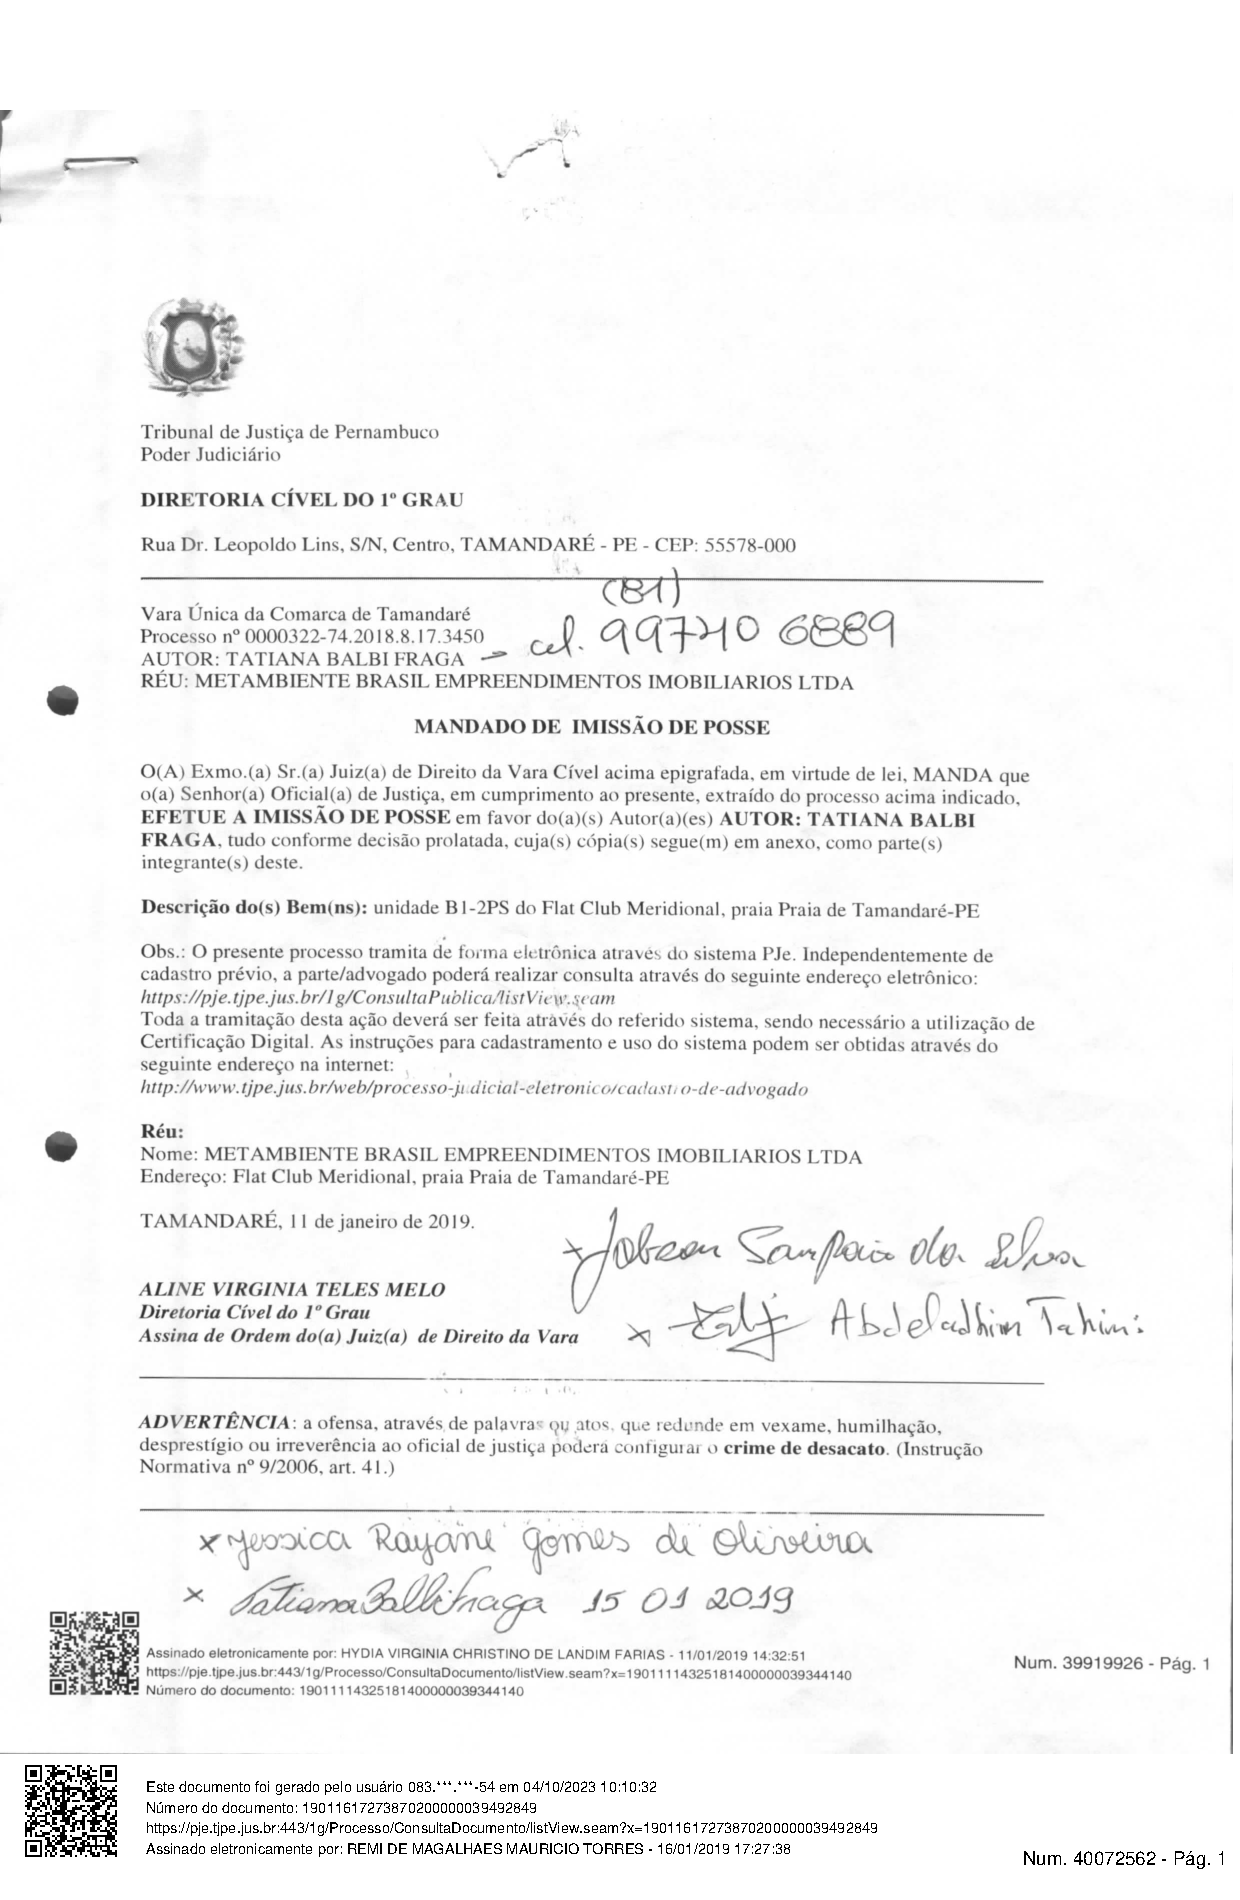
\includepdf[pages=-]{proofs/processo/mandato.pdf}
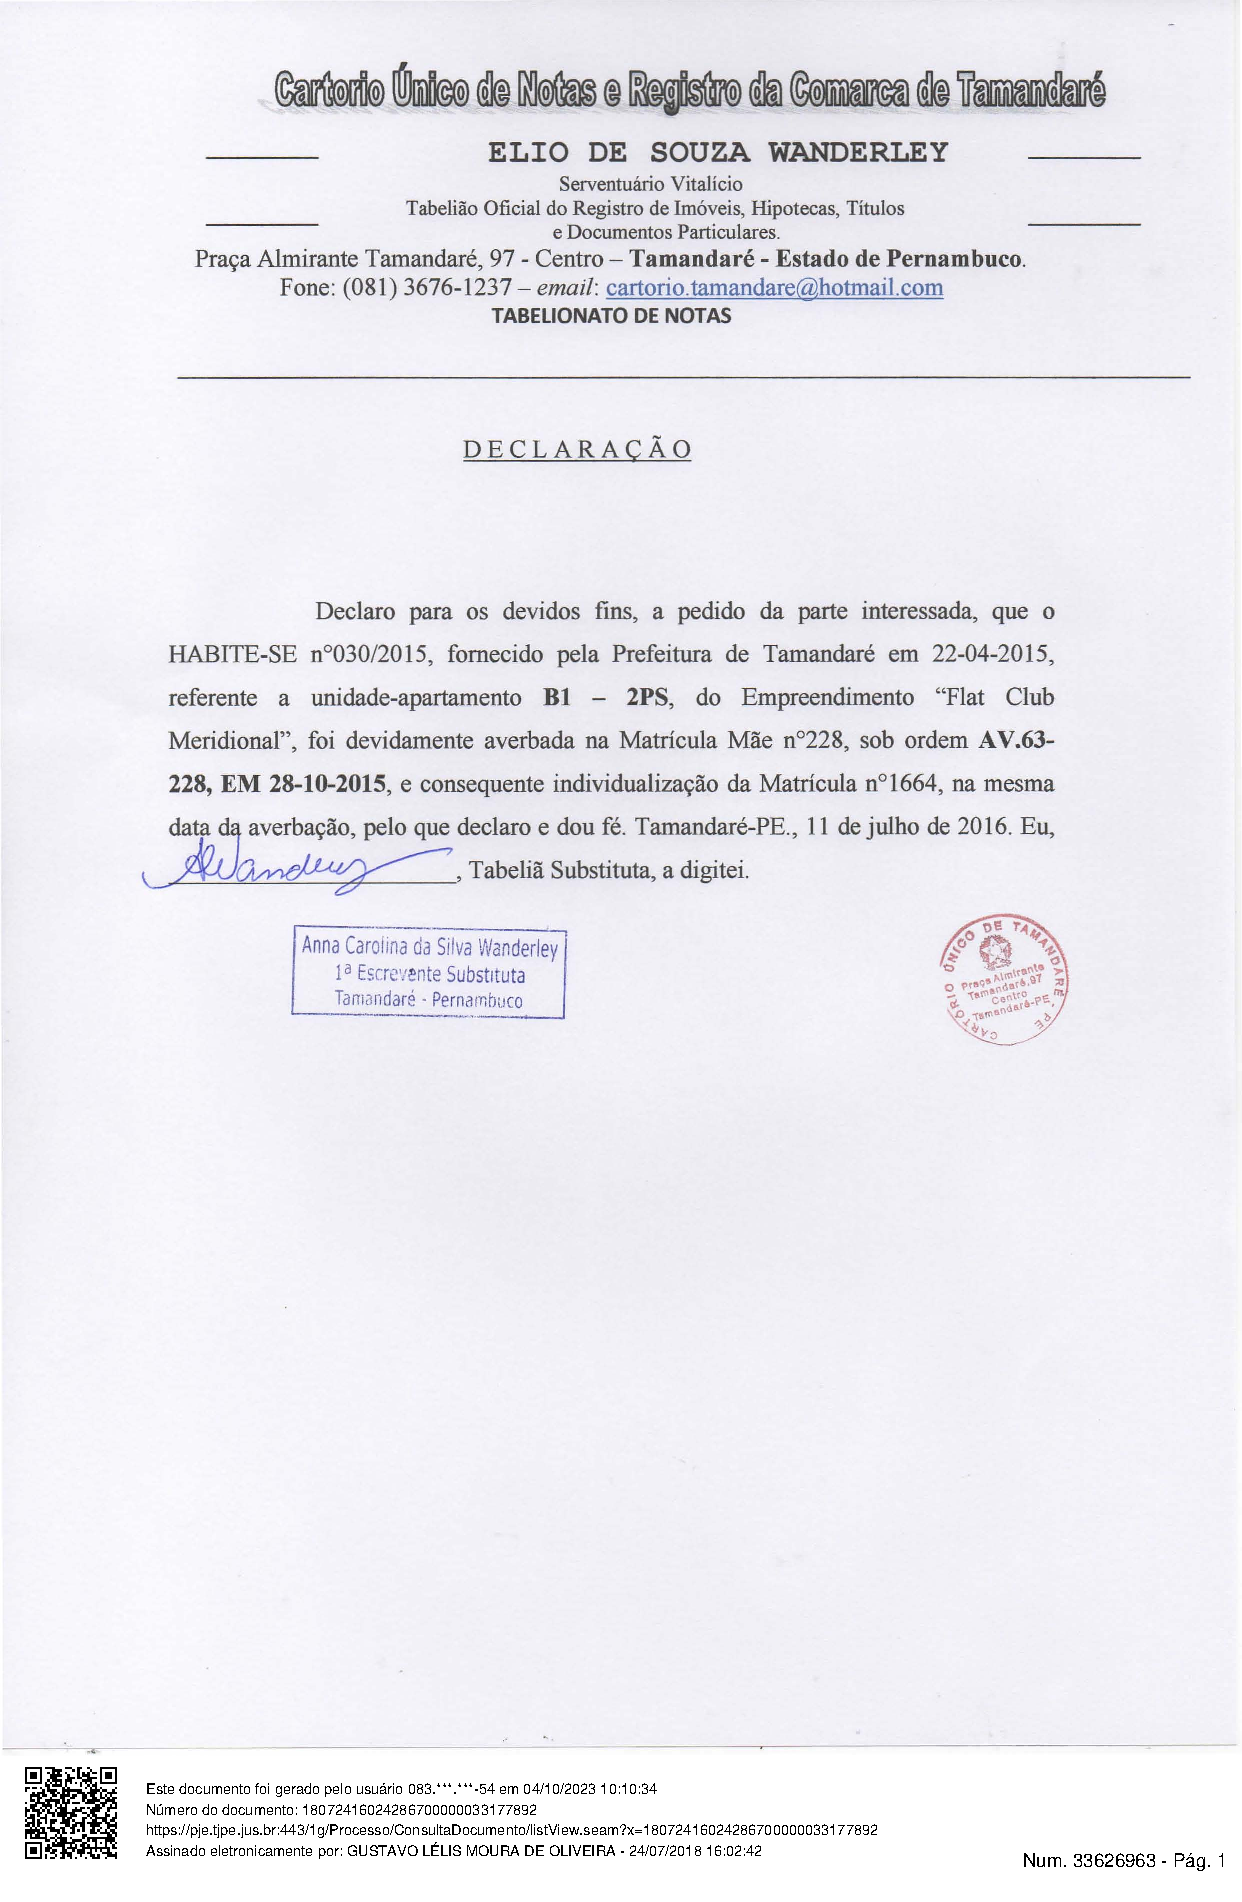
\includepdf[pages=-]{proofs/processo/averbacao.pdf}
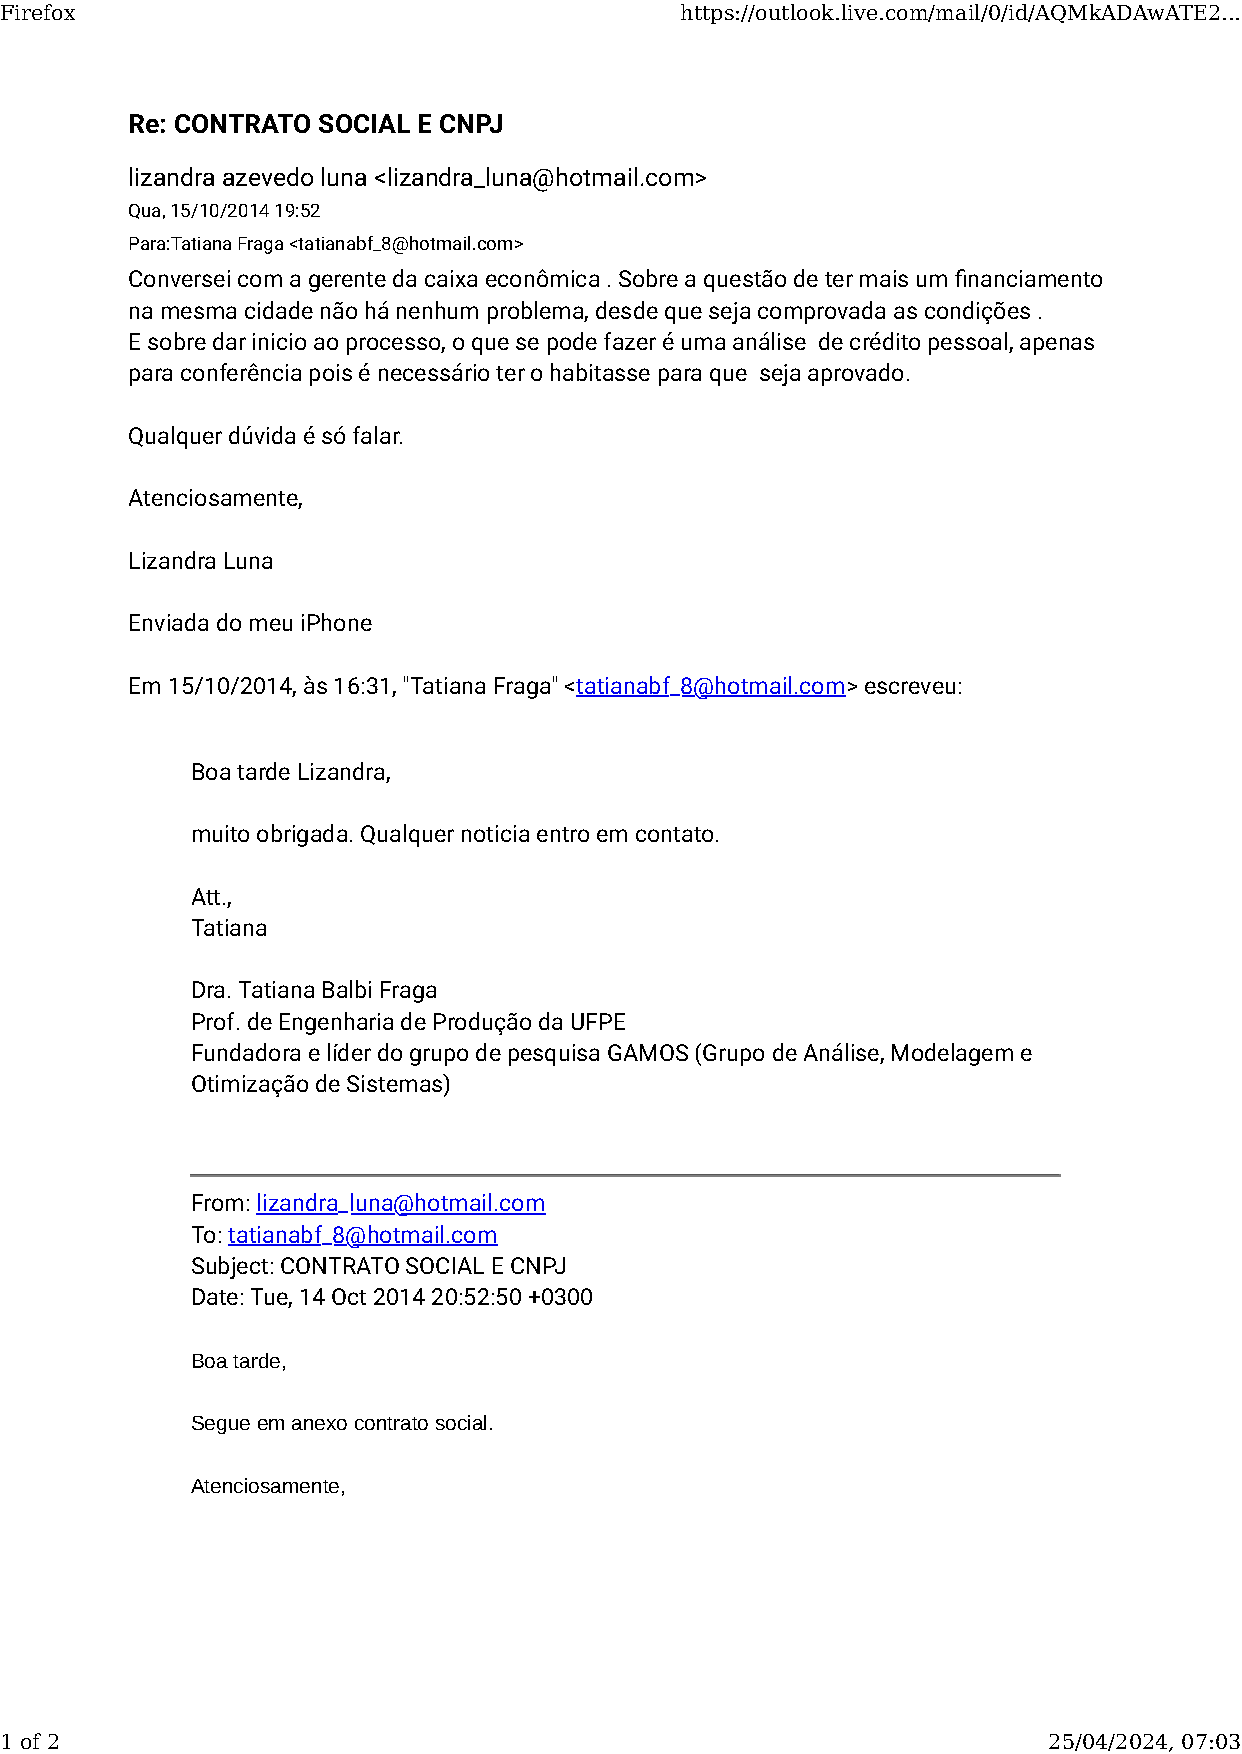
\includepdf[pages=-]{proofs/emails/201410151952.pdf}
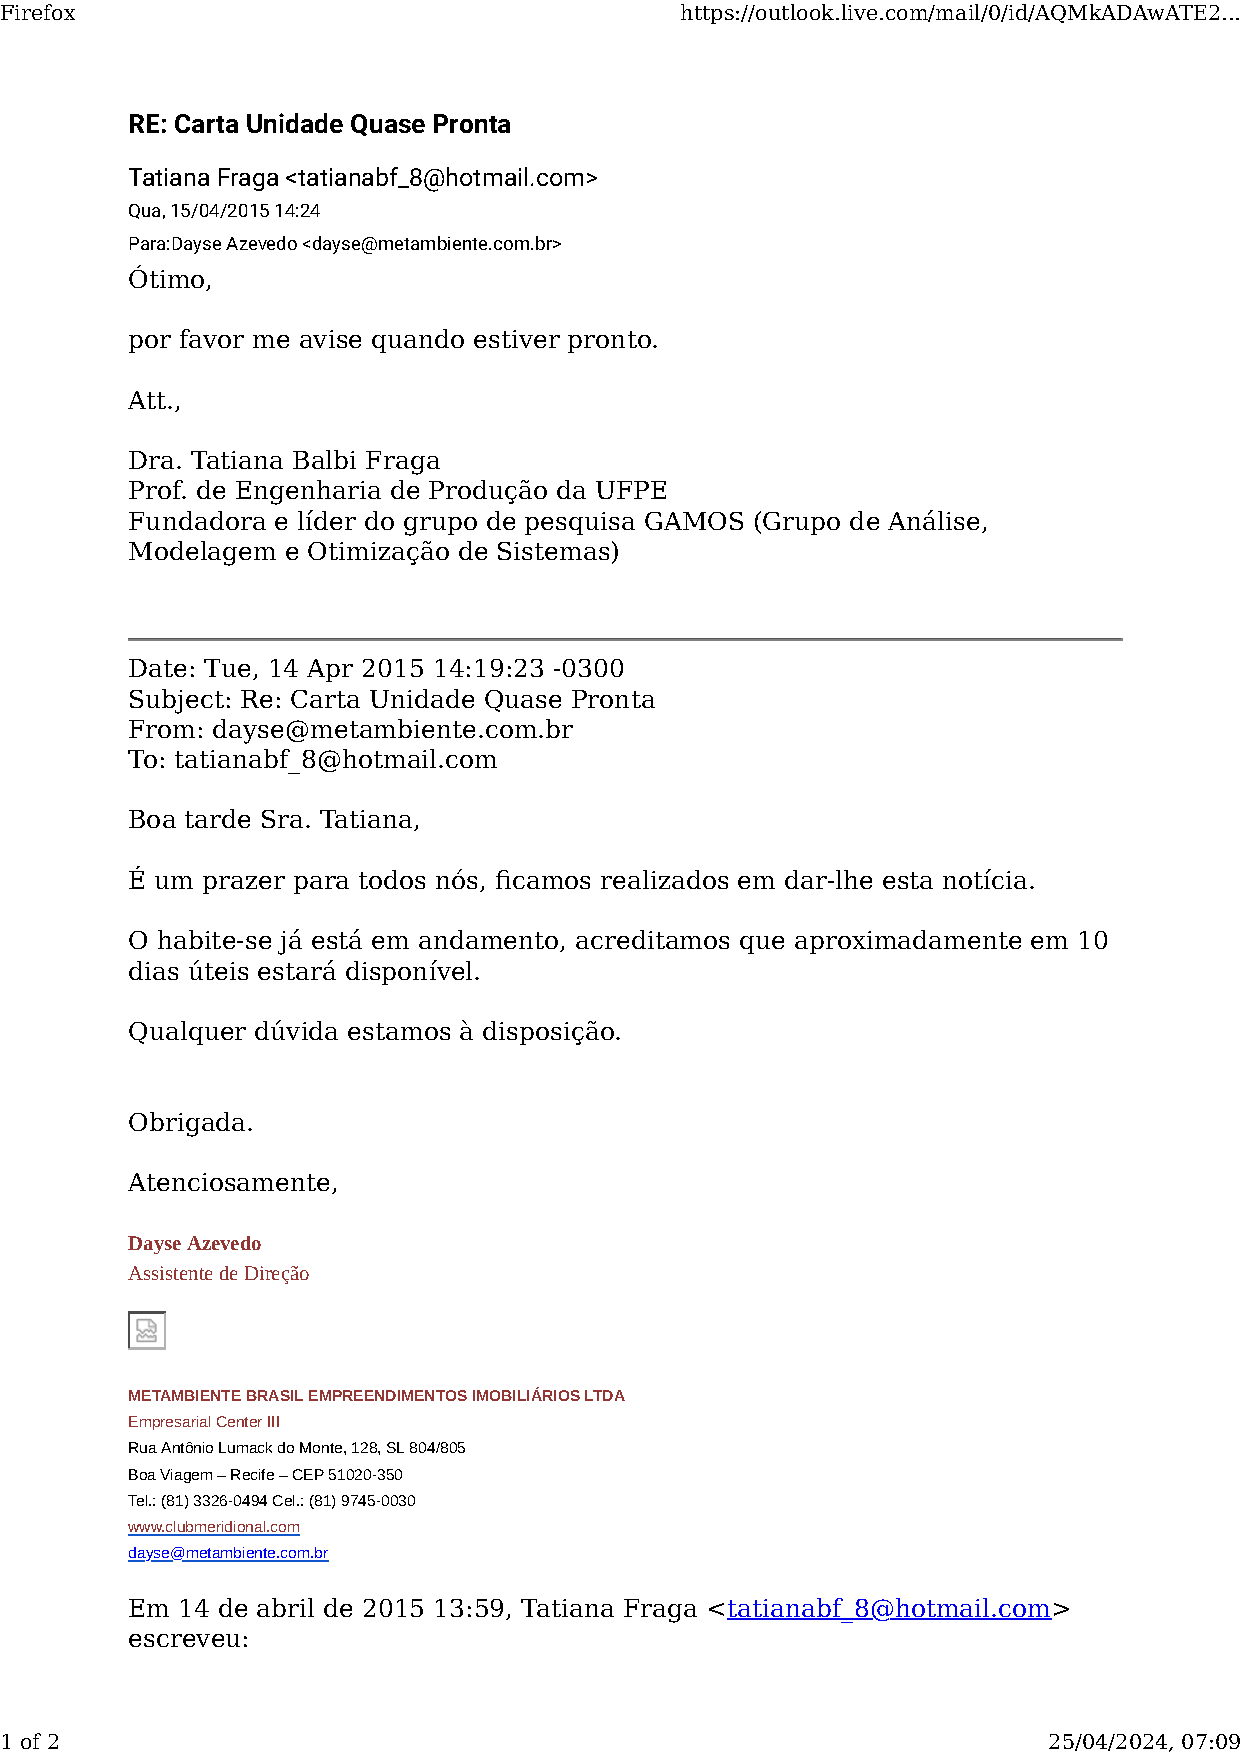
\includepdf[pages=-]{proofs/emails/201504151424.pdf}
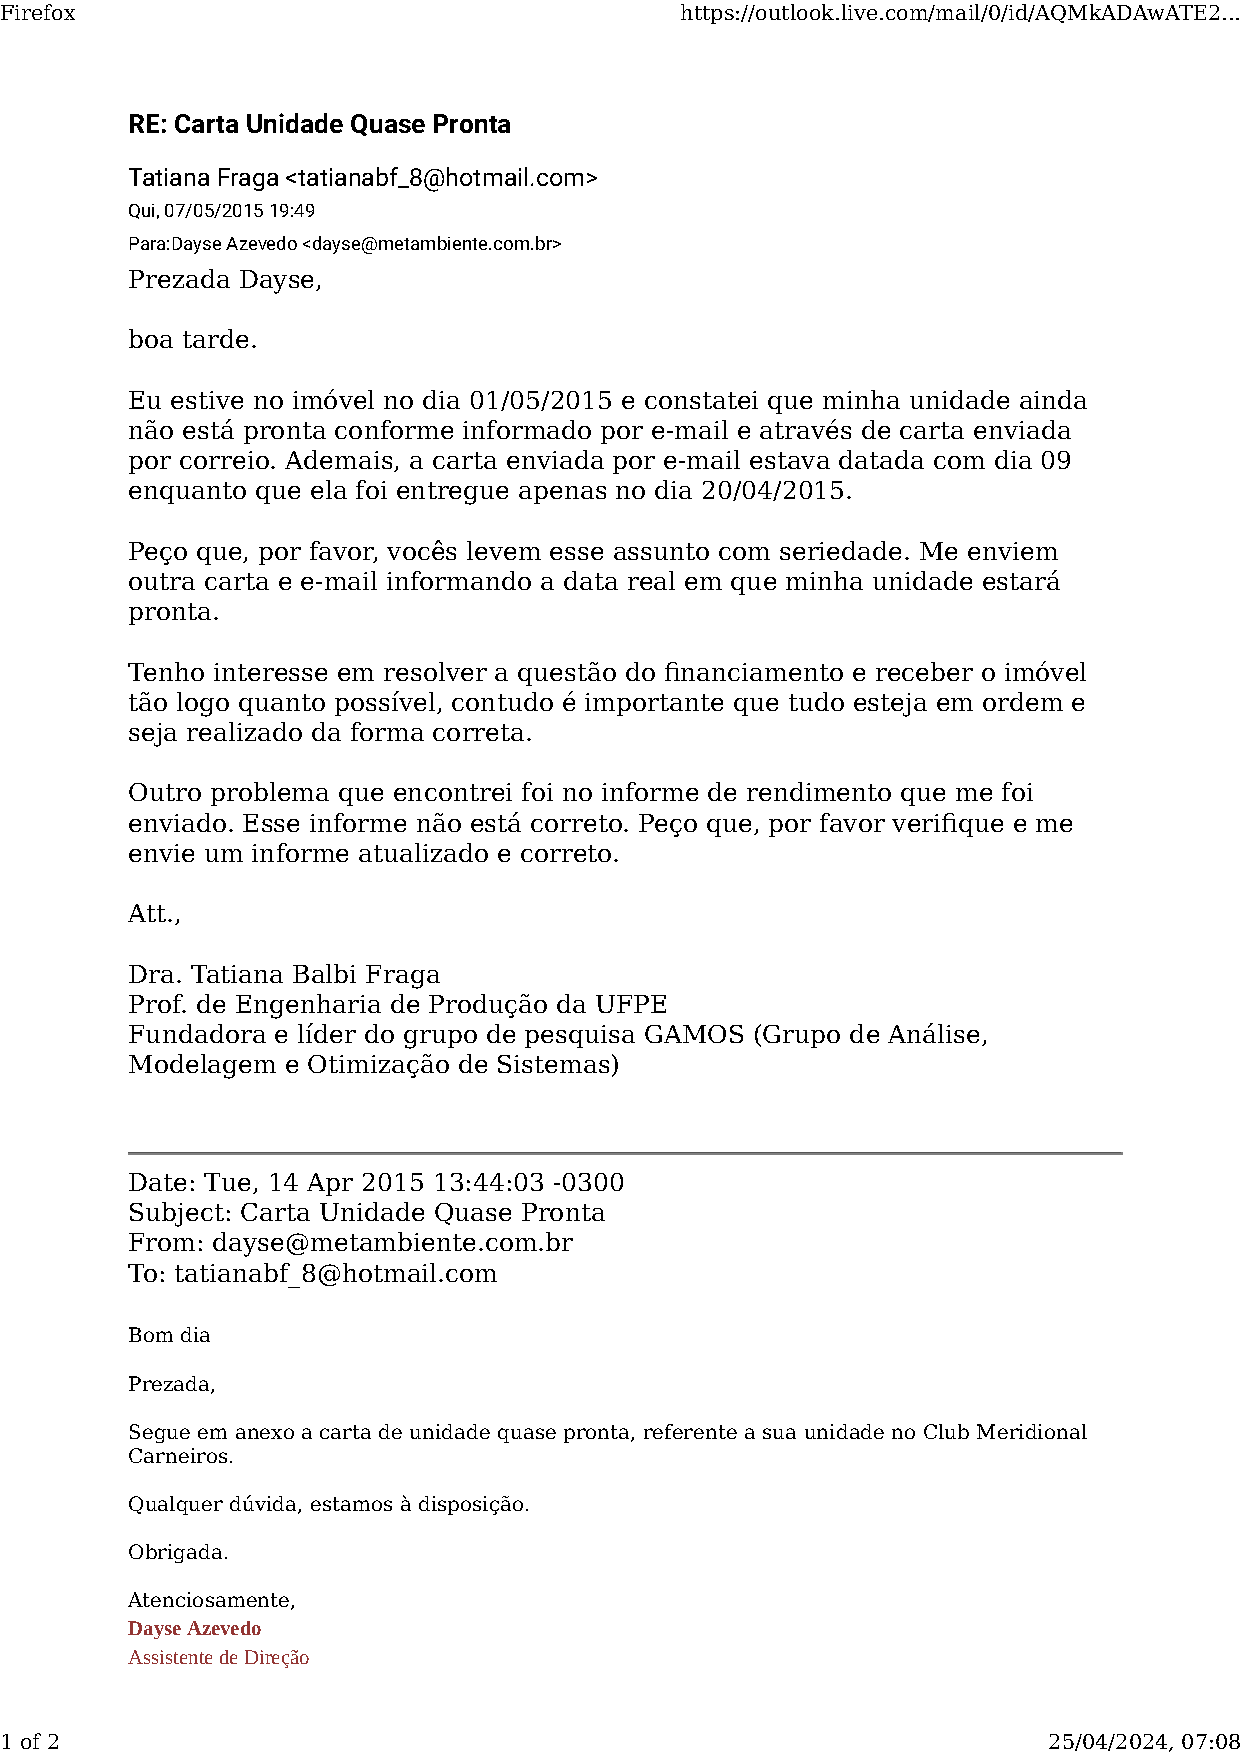
\includepdf[pages=-]{proofs/emails/201505071949.pdf}
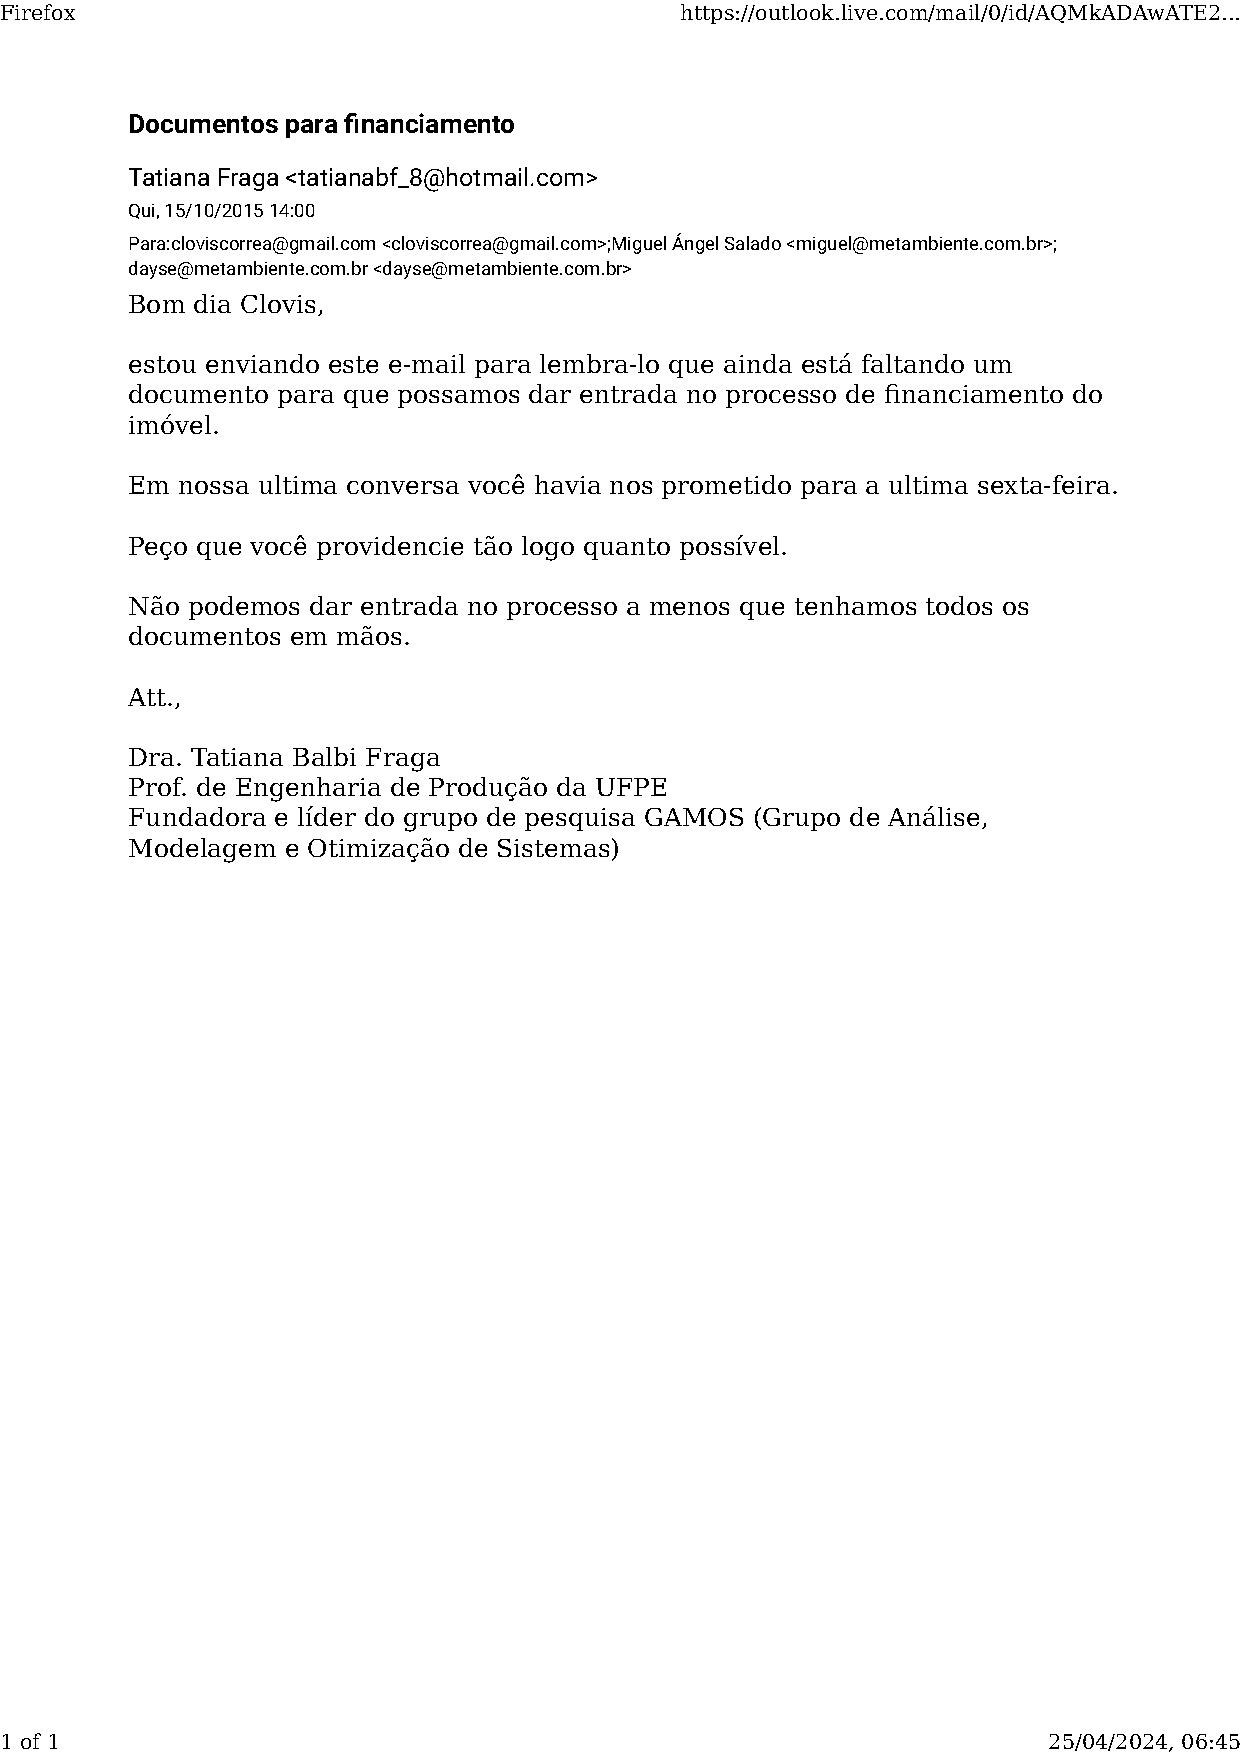
\includepdf[pages=-]{proofs/emails/201510151400.pdf}
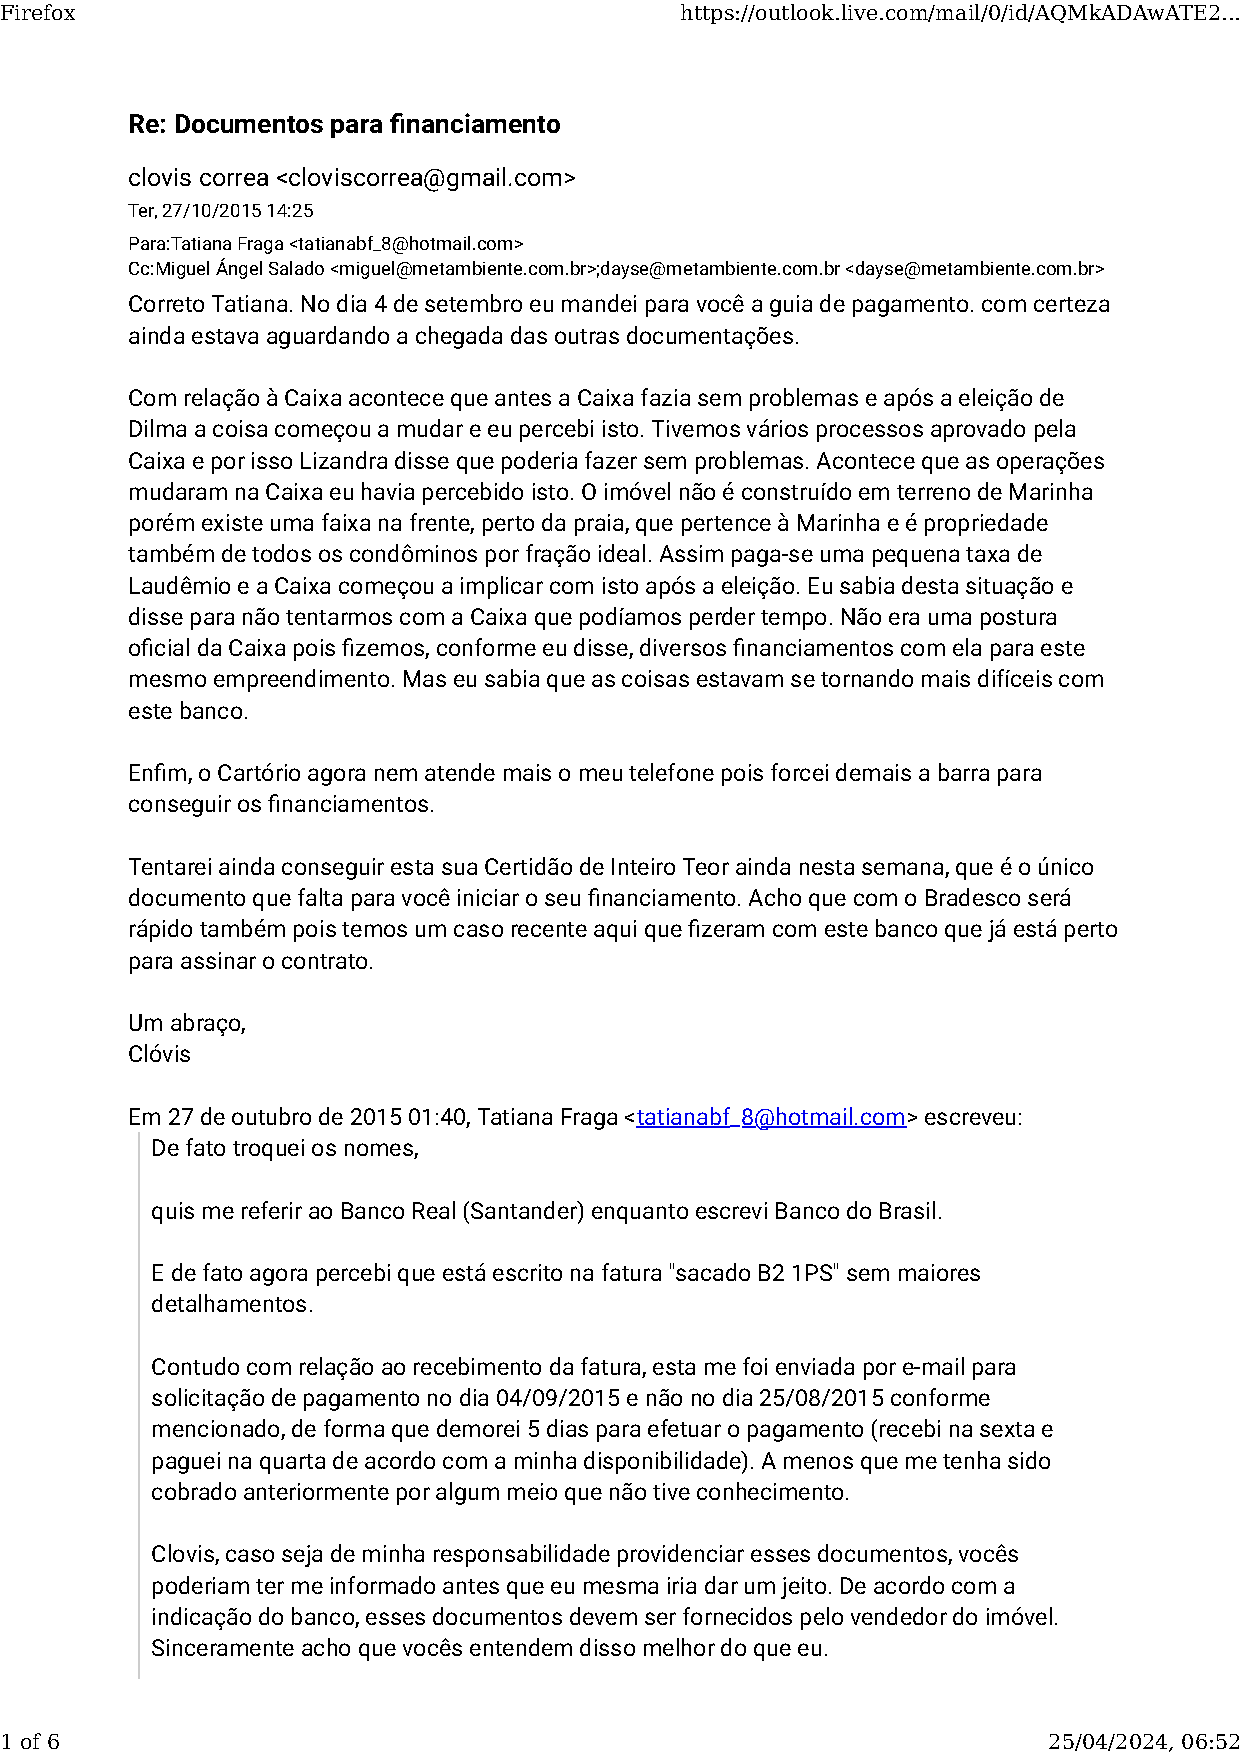
\includepdf[pages=-]{proofs/emails/201510271425.pdf}
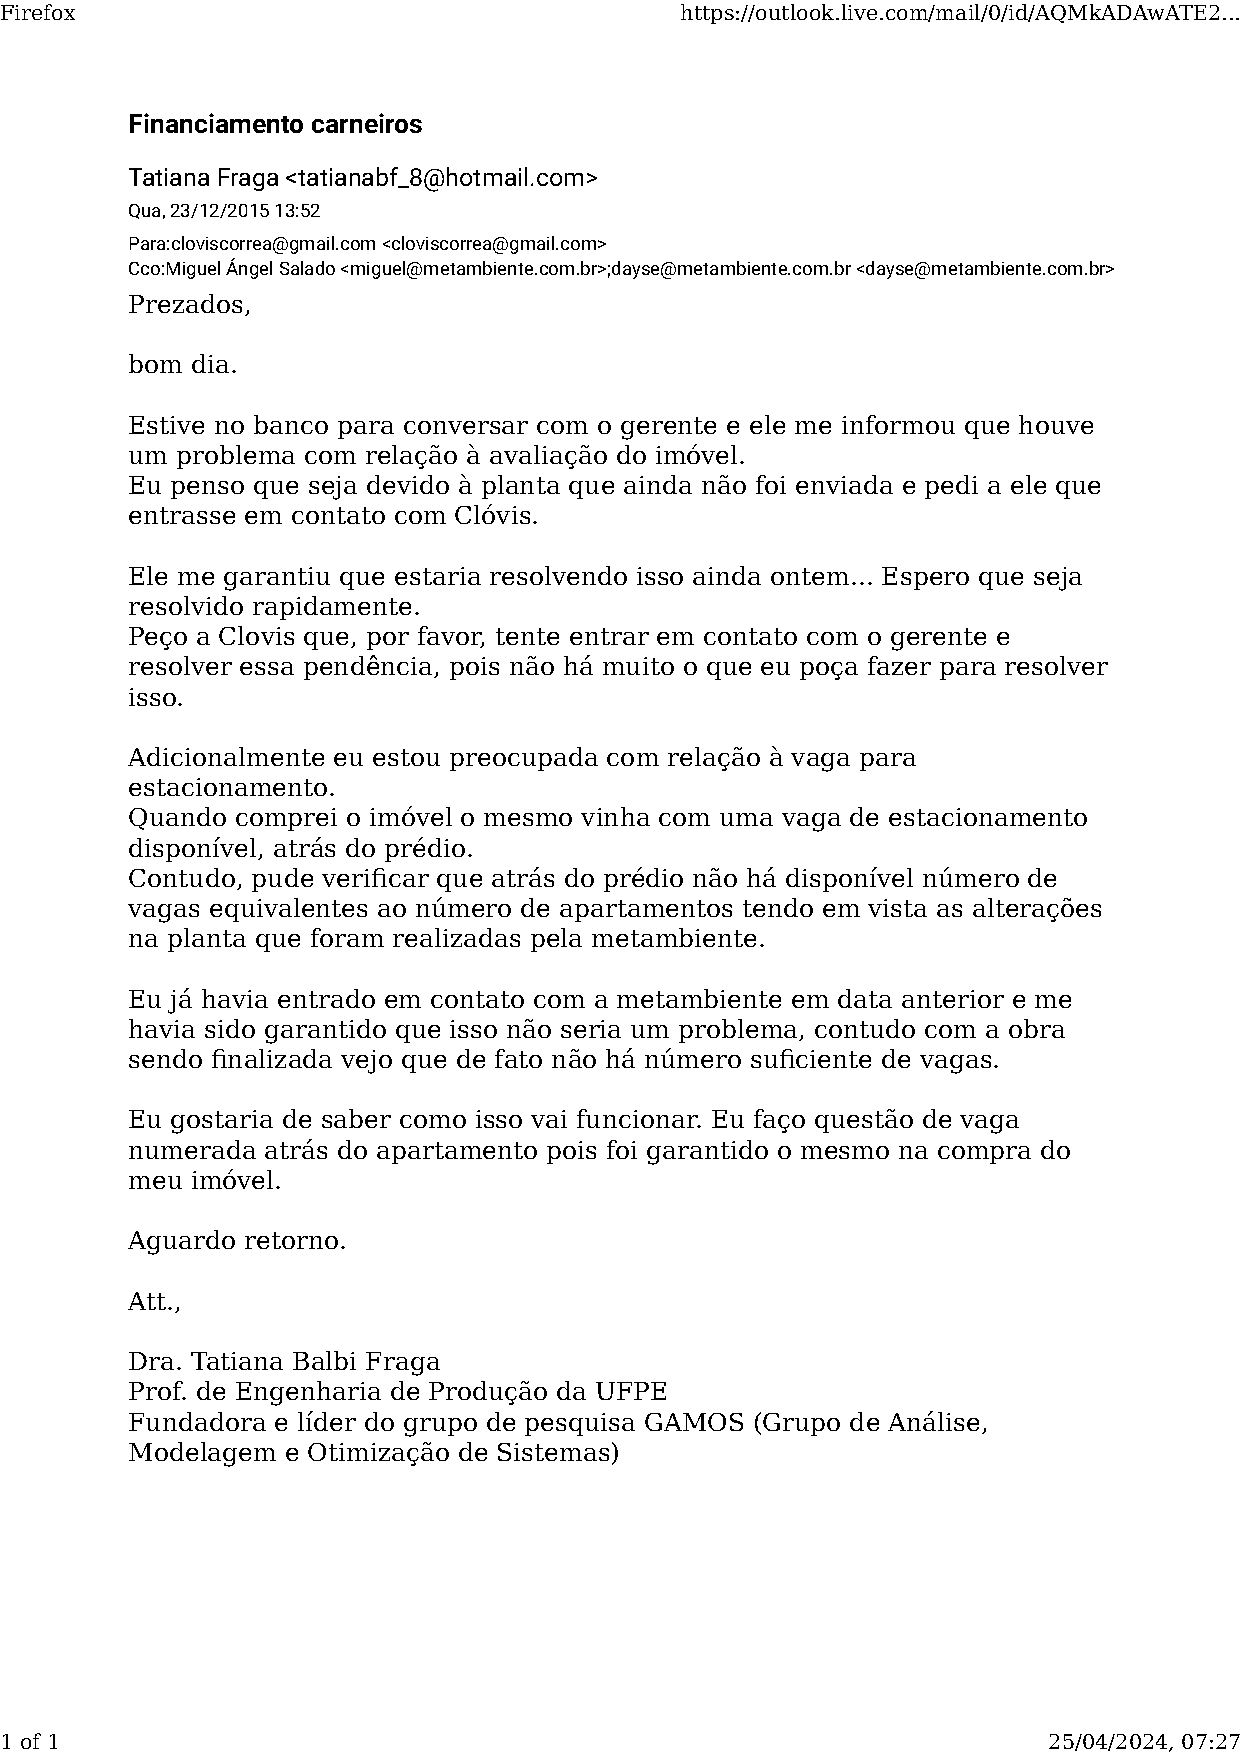
\includepdf[pages=-]{proofs/emails/201512231352.pdf}
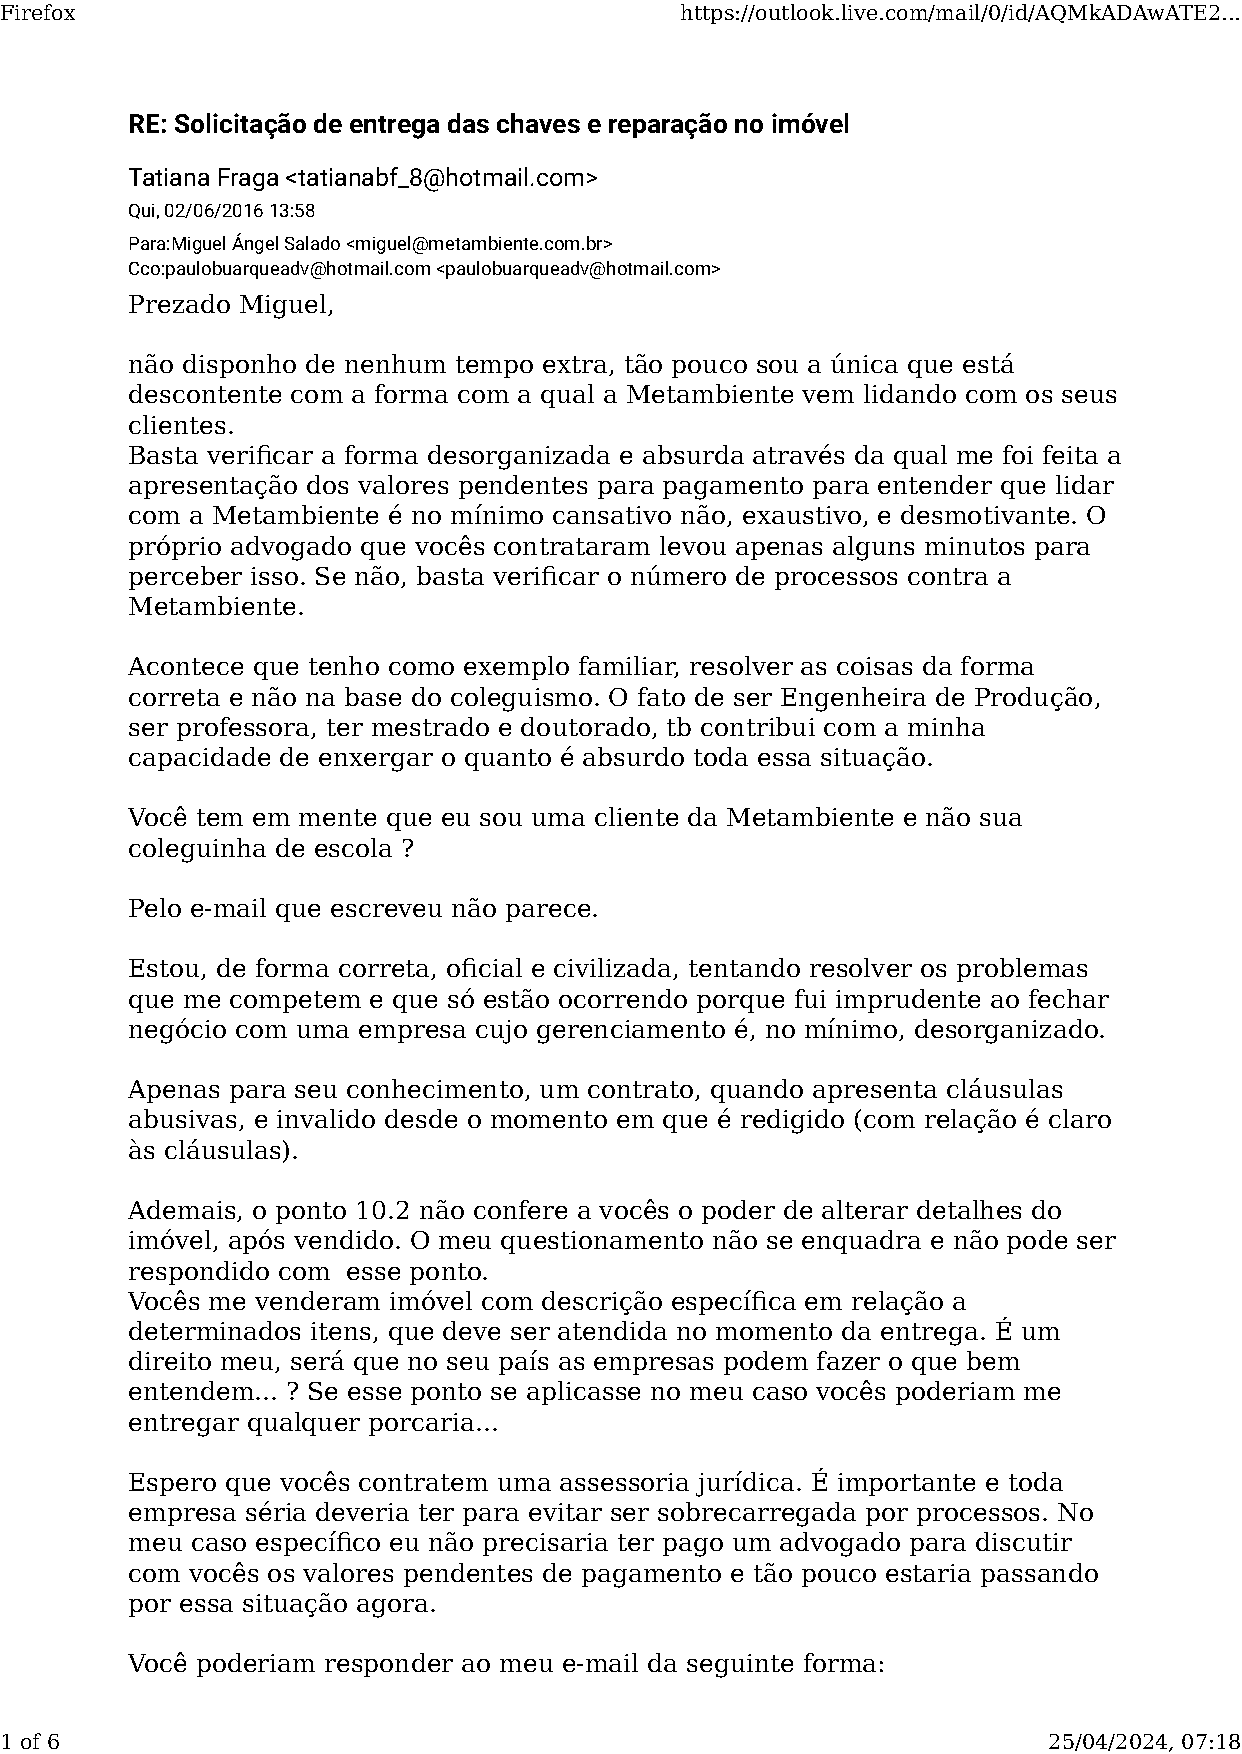
\includepdf[pages=-]{proofs/emails/201606021358.pdf}


\end{document}

